\section{Architektur}
    Unabhängig des verwendeten p2p Übertragungsmediums soll eine Schnittstelle in Form eines auf Requests antwortenden Servers zur Verfügung stehen.

    und sich eine REST Schnittstelle durch die Pakete ...\footnote{TODO} leicht in pharo definieren lässt, bietet es sich an, diese fertigen Serverkomponenten zu nutzen.
    Um REST als Schnittstelle jedoch nutzen zu können muss der genutzte Kommunikationskanal HTTP übertragen können. Da jede der vorgestellten Schnittstellen Bytes oder Strings
    übertragen kann, stellen die Übertragungsmedien kein Problem dar, jedoch muss der REST-Server im Falle von Bluetooth, NFC und USB die HTTP-String Repräsentationen zur Verfügung stellen können,
    ohne sie über eine TCP/IP-Netzwerkschnittstelle zu versenden. Ebenso muss der Client die HTTP-Nachrichten korrekt verarbeiten können.
    Da die meisten Bibliotheken an den TCP/IP-Stack von Android gekoppelt sind, um einen gekapselten HTTP-Client anbieten zu können, ist es nicht immer möglich eine String-Repräsentation des zu tätigenden Aufrufs zu erhalten oder an die Bibliothek zu übergeben.
    Die OkHttp Bibliothek sollte diese Probleme jedoch umgehen können, da Netzwerk Aufrufe durch eine Kette von Interceptoren gereicht werden und der RealNetworkInterceptor,
    welcher sich als letztes in dieser Kette befindet, überschrieben werden kann.\footnote{TODO: gibt OkHttp fertige Http Aufrufe in den letzten Interceptor?}
	Im folgenden wird jedoch nur noch WiFi Direct und damit eine TCP/IP-Implementierung betrachtet.
    Um die Schnittstelle einfach warten zu können, wird sie als JSONSchema über OpenApi dokumentiert und dem Client zur Verfügung gestellt.\footnote{TODO: JSON SCHEMA und OpenApi sollten erklärt werden}

    Die Schnittstelle muss folgende Funktionalitäten anbieten:
    \begin{itemize}
        \item Eine Auflistung der verfügbaren Netzwerkschnittstellen sollte ähnlich zu {\it ip link show} zur Verfügung stehen, um die ID der gewünschten Schnittstelle für die nächsten Aufrufe herauszufinden.
        \item Pro Netzwerkschnittstelle soll es möglich sein, sich den aktuellen Verbindungsstatus sowie die akutelle Konfiguration ausgeben sowie anpassen zu lassen.
        \item Eine Ausgabe von Systemlogs über die Netzwerkschnittstellen soll ungefiltert und pro Schnittstelle gefiltert zur Verfügung stehen.
        \item Die Spezifikation der Schnittstelle soll als Aufruf der Schnittstelle zur Verfügung stehen, sodass sie leicht nutzbar ist.
    \end{itemize}

    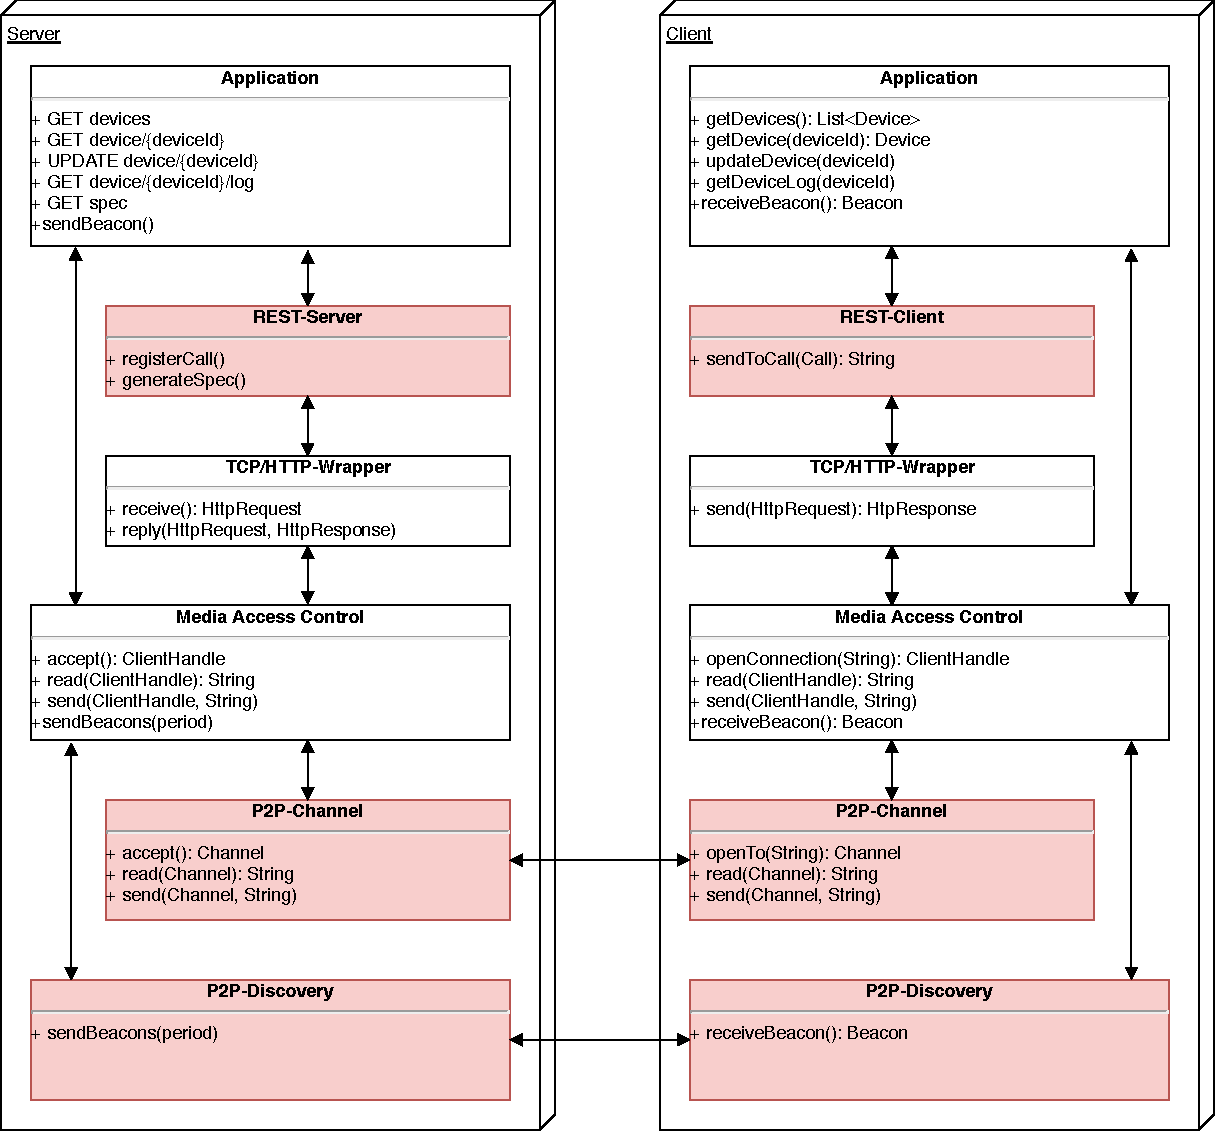
\includegraphics{IOT-Connectivity-Protocol-Stack}

    REFERENCE TO IMAGE zeigt, welche Elemente sich im Protokoll-Stack befinden, um die Serveranwendung als REST-Server Clientgeräten zur Verfügung zu stellen.
    Der REST-Server lässt sich hierbei als eine OpenApi/JsonSchema-Implemnetierung der Zweidenker GmbH nutzen.\footnote{https://github.com/zweidenker/OpenAPI}
